% Options for packages loaded elsewhere
\PassOptionsToPackage{unicode}{hyperref}
\PassOptionsToPackage{hyphens}{url}
%

\documentclass{book}
\usepackage[fontsize=20pt]{fontsize}
\usepackage[a4paper, margin=1in, landscape]{geometry}

%\documentclass[
%]{book}
\usepackage{amsmath,amssymb}
\usepackage{iftex}
\ifPDFTeX
  \usepackage[T1]{fontenc}
  \usepackage[utf8]{inputenc}
  \usepackage{textcomp} % provide euro and other symbols
\else % if luatex or xetex
  \usepackage{unicode-math} % this also loads fontspec
  \defaultfontfeatures{Scale=MatchLowercase}
  \defaultfontfeatures[\rmfamily]{Ligatures=TeX,Scale=1}
\fi
\usepackage{lmodern}
\ifPDFTeX\else
  % xetex/luatex font selection
\fi
% Use upquote if available, for straight quotes in verbatim environments
\IfFileExists{upquote.sty}{\usepackage{upquote}}{}
\IfFileExists{microtype.sty}{% use microtype if available
  \usepackage[]{microtype}
  \UseMicrotypeSet[protrusion]{basicmath} % disable protrusion for tt fonts
}{}
\makeatletter
\@ifundefined{KOMAClassName}{% if non-KOMA class
  \IfFileExists{parskip.sty}{%
    \usepackage{parskip}
  }{% else
    \setlength{\parindent}{0pt}
    \setlength{\parskip}{6pt plus 2pt minus 1pt}}
}{% if KOMA class
  \KOMAoptions{parskip=half}}
\makeatother
\usepackage{xcolor}
\usepackage{longtable,booktabs,array}
\usepackage{calc} % for calculating minipage widths
% Correct order of tables after \paragraph or \subparagraph
\usepackage{etoolbox}
\makeatletter
\patchcmd\longtable{\par}{\if@noskipsec\mbox{}\fi\par}{}{}
\makeatother
% Allow footnotes in longtable head/foot
\IfFileExists{footnotehyper.sty}{\usepackage{footnotehyper}}{\usepackage{footnote}}
\makesavenoteenv{longtable}
\usepackage{graphicx}
\makeatletter
\def\maxwidth{\ifdim\Gin@nat@width>\linewidth\linewidth\else\Gin@nat@width\fi}
\def\maxheight{\ifdim\Gin@nat@height>\textheight\textheight\else\Gin@nat@height\fi}
\makeatother
% Scale images if necessary, so that they will not overflow the page
% margins by default, and it is still possible to overwrite the defaults
% using explicit options in \includegraphics[width, height, ...]{}
\setkeys{Gin}{width=\maxwidth,height=\maxheight,keepaspectratio}
% Set default figure placement to htbp
\makeatletter
\def\fps@figure{htbp}
\makeatother
\setlength{\emergencystretch}{3em} % prevent overfull lines
\providecommand{\tightlist}{%
  \setlength{\itemsep}{0pt}\setlength{\parskip}{0pt}}
\setcounter{secnumdepth}{-\maxdimen} % remove section numbering
\usepackage{fontspec}
\usepackage{xltxtra}
\XeTeXlinebreaklocale "th_TH"
\XeTeXlinebreakskip = 0pt plus 1pt  
\usepackage{fonts-tlwg}

\setmainfont[Script=Thai,%
    Scale=MatchLowercase,%
    WordSpace=1.25,%
    Mapping=tex-text,]{TH Sarabun New}

%% ---- Load line spacing package ---- %%
\usepackage{setspace}

% Introducing hair space 
\newrobustcmd{\hrsp}{\ifmmode\mskip1mu\else\kern0.0625em\fi}





\usepackage{tcolorbox}

% Define a new tcolorbox environment
\newtcolorbox{hello}{
  colframe=red, % border color
  colback=red!10, % background color
  coltext=red, % text color
  boxrule=0.5mm, % border thickness
  left=1mm, % left margin
  right=1mm, % right margin
  top=1mm, % top margin
  bottom=1mm % bottom margin
}
\ifLuaTeX
  \usepackage{selnolig}  % disable illegal ligatures
\fi
\usepackage{bookmark}
\IfFileExists{xurl.sty}{\usepackage{xurl}}{} % add URL line breaks if available
\urlstyle{same}
\hypersetup{
  pdftitle={SCMA104 Systems of Ordinary Differential Equations and Applications in Medical Science},
  pdfauthor={Pairote Satiracoo},
  hidelinks,
  pdfcreator={LaTeX via pandoc}}

\title{SCMA104 Systems of Ordinary Differential Equations and
Applications in Medical Science}
\author{Pairote Satiracoo}
\date{2024-08-18}

\begin{document}
\frontmatter
\maketitle

{
\setcounter{tocdepth}{1}
\tableofcontents
}
\mainmatter
\chapter{หลักการและความสำคัญของแคลคูลัสและระบบสมการเชิงอนุพันธ์สามัญ}\label{uxe2buxe25uxe01uxe01uxe32uxe23uxe41uxe25uxe30uxe04uxe27uxe32uxe21uxe2auxe33uxe04uxe0duxe02uxe2duxe07uxe41uxe04uxe25uxe04uxe25uxe2auxe41uxe25uxe30uxe23uxe30uxe1auxe1auxe2auxe21uxe01uxe32uxe23uxe40uxe0auxe07uxe2duxe19uxe1euxe19uxe18uxe2auxe32uxe21uxe0d}

แคลคูลัสมีส่วนประกอบหลักที่สำคัญอยู่ 2 องค์ประกอบ คือ

\begin{enumerate}
\def\labelenumi{\arabic{enumi}.}
\item
  การหาอนุพันธ์ (differentiation) และ
\item
  การหาปริพันธ์ (Integration)
\end{enumerate}

การประยุกต์เรื่องการหาอนุพันธ์ในการแก้ปัญหาเบื้องต้นที่สำคัญในทางชีววิทยา หรือทางการแพทย์
ประกอบด้วย การหาอัตราการเปลี่ยนแปลงของปริมาณของตัวแปรที่เราสนใจ
และการใช้แคลคูลัสในการแก้ปัญหาการหาค่าสูงสุดและค่าต่ำสุดของปัญหาหรือฟังก์ชันที่แสดงความสัมพันธ์ของตัวแปรที่เราสนใจ

ตัวอย่างการเปลี่ยนแปลงของปริมาณที่สนใจ เช่น ขนาดของประชากร
จำนวนของผู้ติดเชื้อจากโรคทางเดินหายใจ ระดับนำ้ตาลในกระแสเลือด
ปริมาณของยาที่มีอยู่ในกระแสเลือกหรือส่วนหนึ่งของร่างกาย
โดยที่การเปลี่ยนแปลงดังกล่าวสามารถเปรียบเทียบได้กับเวลา ดังต่อไปนี้

\begin{itemize}
\item
  ประชากรในประเทศไทยปี พ.ศ. 2566 มีจำนวน 66.05 ล้านคน (ข้อมูลอ้างอิงจาก
  \href{https://www.boi.go.th/index.php?page=demographic}{สำนักงานคณะกรรมการส่งเสริมการลงทุน})
\item
  ข้อมูลจำนวนผู้รักษาตัวในโรงพยาบาลจากศูนย์ข้อมูล COVID-19 ระหว่างวันที่ 28 กรกฎาคม
  ถึงวันที่ 3 สิงหาคม พ.ศ. 2567 (ข้อมูลอ้างอิงจาก
  \href{https://www.facebook.com/informationcovid19?locale=th_TH}{ศูนย์ข้อมูล
  Covid-19})
\end{itemize}

\begin{figure}

\includegraphics[width=1\linewidth]{images/fig-covid-19} \caption{ข้อมูลจำนวนผู้รักษาตัวในโรงพยาบาลจากศูนย์ข้อมูล COVID-19}\label{fig:fig-covid-19}
\end{figure}

\begin{itemize}
\tightlist
\item
  การเปลี่ยนแปลงของระดับนำ้ตาลในเลือดระหว่างมืออาหารสามมือในหนึ่งวัน (รูปภาพอ้างอิงจาก
  \href{https://en.wikipedia.org/wiki/Blood_sugar_level}{Wikipedia:
  Blood Sugar Level})
\end{itemize}

\begin{figure}
\includegraphics[width=1\linewidth]{images/fig-blood-glucose} \caption{ความผันผวนของระดับน้ำตาลในเลือด (สีแดง) และฮอร์โมนอินซูลิน (สีน้ำเงิน) ในมนุษย์ระหว่างมื้ออาหารสามมื้อ}\label{fig:fig-blood-glucose}
\end{figure}

\begin{itemize}
\tightlist
\item
  การเปลี่ยนแปลงของปริมาณยาในกระแสเลือดที่เวลาต่างๆ สำหรับการให้ยาโดยวิธีต่างๆ
  (รูปภาพอ้างอิงจาก
  \href{https://www.mdpi.com/1420-3049/28/24/8038}{บทความทางวิชาการในฐานข้อมูล
  MDPI})
\end{itemize}

\begin{figure}
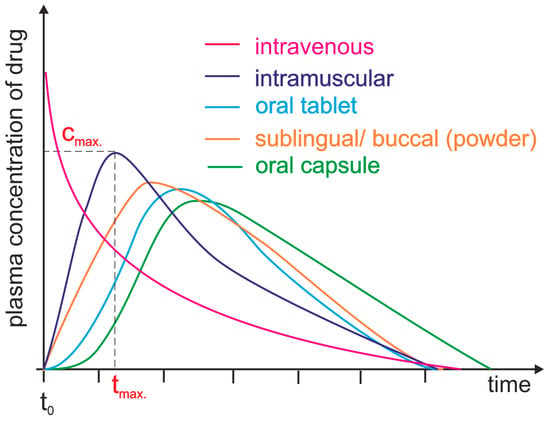
\includegraphics[width=1\linewidth]{images/fig-drug-absorption} \caption{ความเข็มข้นของยาในกระแสเลือดที่เวลาต่างๆ }\label{fig:fig-drug-absorption}
\end{figure}

ในการทำความเข้าใจการเปลี่ยนแปลงของปริมาณข้างต้นเทียบกับเวลา
เราสามารถประยุกต์ใช้การสร้างแบบจำลองทางคณิตศาสตร์เพื่อมาใช้อธิบายการเปลี่ยนแปลงของปริมาณต่างๆ
ที่เกี่ยวข้อง

\begin{quote}
\textbf{การสร้างแบบจำลองทางคณิตศาสตร์} เป็นกระบวนการอธิบายปัญหาหรือ
ปรากฎการต่างๆ ที่เกิดขึ้นในธรรมชาติ โดยปกติแล้วจะอยู่ในรูปของสมการทางคณิตศาสตร์
ซึ่งแบบจำลองทางคณิตศาสตร์นี้จะช่วยให้อธิบายสิ่งต่างๆ ที่เกิดขึ้นในปัญหาหรือปรากฏที่สนใจ
\end{quote}

ตัวอย่างต่อไปนี้จะแสดงถึงแนวคิดในการประยุกต์ของแคลคูลัสที่เกี่ยวข้องกับอัตราการเปลี่ยนแปลงของ

\phantomsection\label{exm1}
ในการทดลองหนึ่ง นักวิจัยต้องการศึกษาการขยายพันธ์ของแบคทีเรียที่มีการการแบ่งตัวที่เรียกว่า
binary fission (การแบ่งตัวแบบทวิภาค) ซึ่งแบคทีเรียจะมีการแบ่งจากหนึ่งเป็นสองเซลเท่าๆ
กัน และได้ผลการทำลองดังต่อไปนี้

\begin{figure}
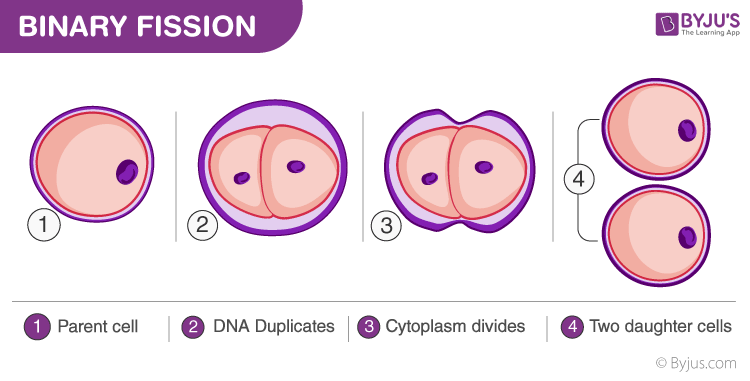
\includegraphics[width=1\linewidth]{images/fig-binary-fission} \caption{กระบวนการแบ่งตัวแบบทวิภาคของแบคทีเรีย}\label{fig:fig-binary-fission}
\end{figure}

(รูปอ้างอิงจาก \href{https://byjus.com/biology/binary-fission/}{BYJU's
Learning Website} )

\begin{longtable}[]{@{}lrrrrrrr@{}}
\caption{จำนวนของแบคทีเรียที่เวลา t ใดๆ}\tabularnewline
\toprule\noalign{}
\endfirsthead
\endhead
\bottomrule\noalign{}
\endlastfoot
เวลา (10 นาที) & 0 & 1 & 2 & 3 & 4 & 5 & 6 \\
จำนวนแบคทีเรีย & 1 & 2 & 4 & 8 & 16 & 32 & 64 \\
\end{longtable}

ตาราง @ref(tab:bacteria-table) และรูปที่ @ref(fig:population-plot)
แสดงการเปลี่ยนแปลงของจำนวนแบคทีเรียที่เวลาใดๆ
ในตัวอย่างนี้การเปลี่ยนแปลงของจำนวนของแบคทีเรียที่เวลา \(t\) สามารถเขียนในรูปฟังก์ชัน
\(N(t)\) ถ้าให้ \(N_0\) แทนจำนวนของแบคทีเรียตอนเริ่มการทดลอง
แล้วแบบจำลองทางคณิตศาสตร์สำหรับการเพิ่มของจำนวนแบคทีเรียจะสามารถเขียนในรูปของสมการ

\begin{equation}
N(t) = N_0 \cdot 2 ^t, \quad t = 0,1,2, \ldots
(\#eq:population-growth)
\end{equation}

ในแบบจำลองทางคณิตศาสตร์นี้การเปลี่ยนแปลงของจำนวนแบคทีเรียที่เวลา \(t\) ใดๆ
เพิ่มขึ้นในลักษณะที่เรียกว่า เอกซ์โพเนนเชียล (Exponential Population Growth)

\begin{figure}
\centering
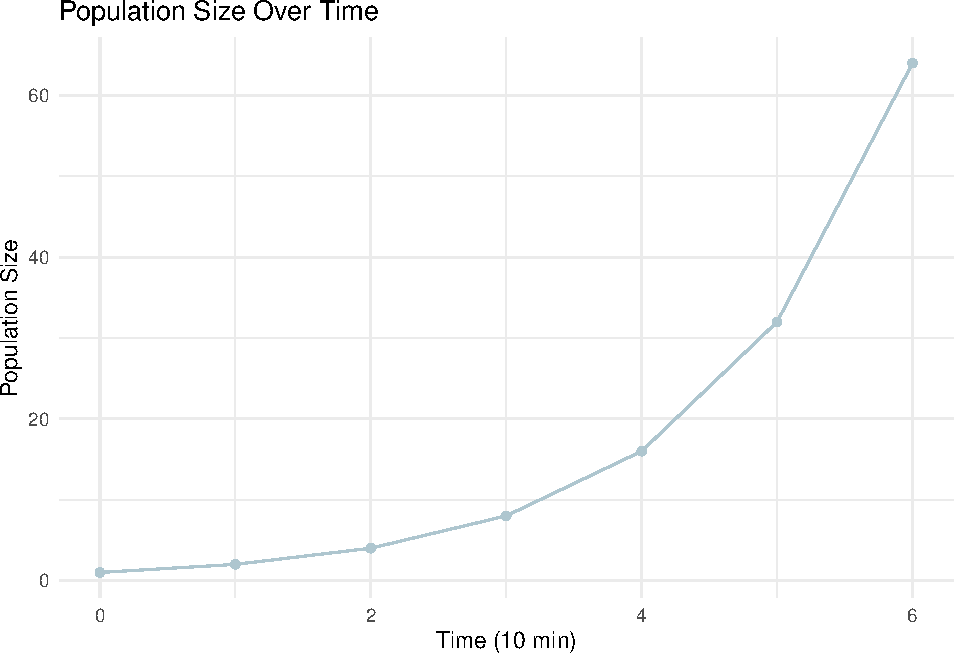
\includegraphics{SCMA104bookdownproj_files/figure-latex/population-plot-1.pdf}
\caption{Population Size Over Time}
\end{figure}

\phantomsection\label{exm2}
ในการสร้างแบบจำลองทางคณิตศาสตร์ ในตัวอย่างของการขยายพันธ์แบคทีเรีย หรือในปัญหาอื่นๆ
แทนที่เราจะพยายามหาความสัมพันธ์ หรือฟังก์ชัน \(N(t)\) ในรูปของเวลา \(t\) โดยตรง
ถ้าเราทราบกระบวนการที่เกี่ยวข้องกับการอัตราการเปลี่ยนแปลงของตัวแปร \(N(t)\) นั้น
เราสามารถนำมาใช้ในการสร้างแบบจำลองทางคณิตศาสตร์ ได้ดังต่อนี้
กระบวนการที่เกี่ยวข้องกับการเปลี่ยนแปลงของจำนวนแบคทีเรีย (การเพิ่มหรือลดลงของแบคทีเรีย)
ที่เกิดขึ้นในระหว่างเวลา \(t\) และเวลา \(t + h\) เกิดจากจำนวนแบคทีเรียที่เพิ่มขึ้น
(เกิดขึ้นมาใหม่) ในช่วงเวลาดังกล่าว และลดลงจากจำนวนแบคทีเรียที่ลดลง (ตายไป)
ในช่วงเวลาดังกล่าวเช่นกัน ซึ่งเราสามารถเขียนในรูปของสมการได้ดังต่อไปนี้

\begin{align}
N(t + h) &= N(t) \\
&\quad + \text{จำนวนแบคทีเรียที่เกิดขึ้นใหม่ระหว่าง } t \text{ และ } t+h \\
&\quad - \text{จำนวนแบคทีเรียที่ตายไประหว่าง } t \text{ และ } t+h
(\#eq:population-growth-2)
\end{align}

ในที่นี้ ``\textbf{การเกิด}'' เราหมายถึงการเพิ่มจำนวนของแบคทีเรียจากหนึ่งเป็นสอง
และเราจะกำหนดให้ \(h\) เป็นช่วงเวลาสั้นๆ
(ซึ่งเราสามารถใช้ความรู้แคลคูลัสในการสร้างแบบจำลองทางคณิตศาสตร์ในรูปของสมการเชิงอนุพันธ์
(differential equation)) ในสมการ @ref(eq:population-growth-2)
ถ้าเราสมมติว่า การเพิ่มของแบคทีเรียเป็นสัดส่วนกับจำนวนแบคทีเรียที่มีอยู่ในขณะนั้น
หรือเขียนในรูปของสมการได้ดังนี้

\[
\text{จำนวนแบคทีเรียที่เกิดใหม่ระหว่าง } t \text{ และ } t + h \approx b \cdot N \cdot h
\]

\[
\text{จำนวนแบคทีเรียที่ตายไประหว่าง } t \text{ และ } t + h \approx m \cdot N \cdot h
\]

โดยที่ค่าคงตัว \(b\) และ \(m\) ในสมการข้างต้น คือ อัตราการเกิด (birth rate)
และอัตราการตาย (mortality rate)

เมื่อแทนจำนวนแบคทีเรียที่เกิดใหม่ และตายไประหว่างช่วงเวลาที่กำหนดลงในสมการ
@ref(eq:population-growth-2) จะได้สมการ

\begin{equation}
N(t + h) - N(t) = b\cdot N(t) \cdot h - m\cdot N(t) \cdot h
(\#eq:population-growth-3)
\end{equation}

เราสามารถจัดรูปสมการ @ref(eq:population-growth-3)
ได้ไหมในรูปของ\textbf{อัตราการเปลี่ยนแปลงเฉลี่ย}ของจำนวนแบคทีเรียในช่วงเวลาดังกล่าว
ดังนี้

\begin{align}
\frac{N(t + h) - N(t)}{h} &= b\cdot N(t)  - m\cdot N(t)\\
(\#eq:population-growth-4)
\end{align}

ดังนั้น ถ้าเราให้ \(h\) เข้าใกล้ 0 ผ่านการหาค่าลิมิต เราจะได้อัตราการเปลี่ยนแปลงขณะหนึ่ง
(instantaneous rate of change) และเขียนได้ในรูปของสมการเชิงอนุพันธ์ ดังนี้

\begin{align}
\frac{dN}{dt} = \lim_{h \rightarrow 0}\frac{N(t + h) - N(t)}{h} &= b\cdot N(t)  - m\cdot N(t)\\
(\#eq:population-growth-5)
\end{align}

ทั้งนี้ในการแก้สมการเชิงอนุพันธ์ @ref(eq:population-growth-5)
เพื่อให้ได้คำตอบที่แสดงจำนวนแบคทีเรีย \(N(t)\) ในรูปของฟังก์ชันของ \(t\)
เราจะต้องกำหนดเงื่อนไขเพิ่มเติมที่เกี่ยวข้องกับจำนวนแบคทีเรีย \(N(t)\) ที่เวลา \(t\) หนึ่ง
โดยทั่วไปเราจะกำหนดค่าเริ่มต้นของจำนวนแบคทีเรียที่ \(t = 0\) ดังนั้น
ถ้าเรากำหนดเงื่อนไขเริ่มต้น (initial condition)

\begin{equation}
N(0) = N_0
(\#eq:population-growth-6)
\end{equation}

เราสามารถหาคำตอบของสมการเชิงอนุพันธ์ที่มีเงื่อนไขเริ่มต้นโดยวิธีการหาปริพันธ์
(Integration) ได้คำตอบของสมการดังนี้

\begin{equation}
N(t) = N_0 e^{(b-m)t}
(\#eq:population-growth-7)
\end{equation}

\phantomsection\label{exm3}
ในการทดลองเลี้ยงยีสต์ในขวดทดลองที่มีอาหารเลี้ยงยีสต์ในปริมาณที่เหมาะสม
ผู้ทำการทดลองสนใจที่จะประมาณค่าของยีสต์โดยอาศัยแบบจำลองการเปลี่ยนแปลงของประชากรที่อธิบายด้วยสมการ
@ref(eq:population-growth-7) กำหนดให้

\begin{itemize}
\item
  ภายใต้สภาวะของการทดลองที่เหมาะสม ยีสต์จะแบ่งตัวทุกๆ 90 นาที
\item
  ยีสต์มีครึ่งชีวิตเท่ากับ 1 สัปดาห์
\end{itemize}

จากข้อมูลดังกล่าว จงแสดงวิธีทำเพื่อหาคำตอบจากคำถามต่อไปนี้

\begin{enumerate}
\def\labelenumi{\arabic{enumi}.}
\item
  จงประมาณค่าของอัตราการเกิด \(b\) (1/ชั่วโมง) และอัตราการตาย \(m\) (1/ชั่วโมง)
\item
  เขียนแบบจำลองทางคณิตศาสตร์โดยใช้ค่า \(b\) และ \(m\) ที่ประมาณค่าได้ (สมการ
  @ref(eq:population-growth-7))
\item
  ใช้เครื่องมือที่นักศึกษามีอยู่ในการวาดกราฟแสดงความสัมพันธ์ของจำนวนยีสต์ที่เวลาต่างๆ
\item
  เปรียบเทียบผลลัพธ์ที่ได้กับรูปภาพแสดงการเปลี่ยนแปลงของยีสต์จากการทดลองในห้องปฏิการ
  ตามรูปที่ @ref(fig:fig-yeast-cells) (รูปภาพอ้างอิงจาก
  \href{https://homework.study.com/explanation/a-graph-of-a-population-of-yeast-cells-in-a-new-laboratory-culture-as-a-function-of-time-is-shown-a-describe-how-the-rate-of-population-increase-varies-b-when-is-this-rate-highest-c-on-what-intervals-is-the-population-function-concave-upward-or-d.html}{https://homework.study.com/})
\end{enumerate}

\begin{figure}
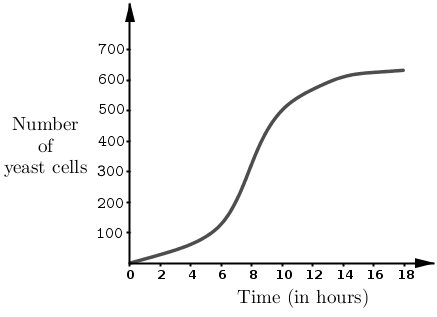
\includegraphics[width=0.5\linewidth]{images/fig-yeast-cells} \caption{กราฟการเจริญเติบโตของเซลล์ยีสต์}\label{fig:fig-yeast-cells}
\end{figure}

\phantomsection\label{exm4}
จงใช้อินเทอร์เน็ตเพื่อค้นหาตัวอย่างแบบจำลองทางคณิตศาสตร์ที่อธิบายโดยสมการเชิงอนุพันธ์หรือระบบสมการเชิงอนุพันธ์
ข้อมูลที่ต้องการประกอบด้วย

\begin{enumerate}
\def\labelenumi{\arabic{enumi}.}
\item
  ค้นหาหน้าเว็บที่ให้ข้อมูลเกี่ยวกับแบบจำลองทางคณิตศาสตร์ในปัญหาที่นักศึกษาสนใจ
\item
  จดบันทึก URL ของหน้าเว็บ
\item
  เขียนสรุปสั้นๆ ว่าโมเดลนี้ใช้เพื่ออะไร
\end{enumerate}

โดยสรุป แคลคูลัสและสมการเชิงอนุพันธ์เป็นเครื่องมือสำคัญในการทำความเข้าใจว่าสิ่งต่างๆ
เปลี่ยนแปลงไปอย่างไรและ แคลคูลัสช่วยให้เราวิเคราะห์อัตราการเปลี่ยนแปลงและพื้นที่ใต้เส้นโค้ง
ในขณะที่สมการเชิงอนุพันธ์ช่วยให้เราสร้างแบบจำลองระบบที่ซับซ้อนในสาขาต่างๆ เช่น ฟิสิกส์
วิศวกรรม เศรษฐศาสตร์ และชีววิทยา
แนวคิดทางคณิตศาสตร์เหล่านี้มีความสำคัญต่อการแก้ปัญหาในโลกแห่งความเป็นจริง
เมื่อโลกของเราก้าวหน้ามากขึ้น
ความสำคัญของแคลคูลัสและสมการเชิงอนุพันธ์ก็จะเพิ่มขึ้นอย่างต่อเนื่อง
ซึ่งสนับสนุนความก้าวหน้าทางวิทยาศาสตร์และเทคโนโลยี

\chapter{ลิมิต (Limits)}\label{uxe25uxe21uxe15-limits}

อาจกล่าวได้ว่า วิชาแคลคูลัส
ถือกำเนิดขึ้นมาจากความพยายามในการแก้ปัญหาทางเรขาคณิตบนระนาบ 2 ปัญหาหลักๆ คือ

\begin{itemize}
\item
  การหาเส้นตรงที่สัมผัสเส้นโค้งที่กำหนดให้

  กำหนดฟังก์ชัน (function) \(f\) และกำหนดจุด \(P(x_{0},y_{0})\) บนกราฟ
  \(y = f(x)\) จงหาสมการของเส้นตรงที่สัมผัสกราฟ \(y = f(x)\) ที่จุด \(P\)
\item
  การหาพื้นที่ของบริเวณที่กำหนดให้

  กำหนด function \(f\) และช่วง \([a,b]\) ในโดเมนของ \(f\)
  จงหาพื้นที่ที่ถูกปิดล้อมด้วยแกน \(X\) และกราฟ \(y = f(x)\) สำหรับ \(x \in [a,b]\)
\end{itemize}

แนวความคิดในการแก้ปัญหาทั้งสอง นำไปสู่การศึกษาเรื่อง ลิมิต (Limits)
ซึ่งเป็นพื้นฐานของวิชาแคลคูลัสนั่นเอง

แต่ในปัจจุบันเราพบว่าวิชาแคลคูลัสมีประโยชน์ในการช่วยแก้ปัญหาในสาขาวิชาต่าง ๆ มากมาย เช่น
เราจะพบในการศึกษาวิชานี้ว่า แคลคูลัสมีบทบาทในการแก้ปัญหาต่อไปนี้

\begin{itemize}
\item
  โดยทั่วไป ยาชนิดฉีดจะต้องใช้เวลาระยะหนึ่งหลังจากฉีดเข้าสู่ร่างกาย
  ในการที่จะไหลเวียนในกระแสโลหิต จนกระทั่งมีความเข้มข้นสูงสุด สมมุติว่า
  ยาฉีดชนิดหนึ่งหลังจากฉีดเข้าสู่ร่างกายนาน \(t\) ชั่วโมง จะมีความเข้มข้นเป็น
  \(C(t) = 0.15(e^{-0.18t}-e^{-1.2t})\) มิลลิกรัมต่อมิลลิลิตร จงหาว่า
  นานเท่าใดหลังจากฉีดยา จึงจะมีความเข้มข้นของยา ในกระแสโลหิตสูงที่สุด
\item
  เราอาจประมาณได้อย่างมีเหตุผลว่า artery มีรูปร่างที่เป็นผลมาจากการหมุนรอบแกน
  ของเส้นโค้งในระนาบ โดยในสภาวะนิ่ง รัศมีของ artery มีค่าคงที่เท่ากับ 1 หน่วย
  (รูปทรงกระบอก) แต่ในขณะที่หัวใจสูบฉีดโลหิตผ่าน artery artery จะพองตัวออก
  ทำให้รัศมีเปลี่ยนไปตามสมการ \(R(x) = 1+0.4x-0.04x^{2}\) หน่วย เมื่อ
  \(0 \leq x\leq 10\) เป็นตำแหน่งบนแนวยาวของ artery จงหาว่า ปริมาณโลหิตที่อยู่ใน
  artery ขณะที่หัวใจสูบฉีดโลหิตผ่านเข้ามาเป็นกี่เท่าของความจุโลหิตในสภาวะนิ่ง
\item
  ความก้าวหน้าในทางการแพทย์ และเทคโนโลยีปัจจุบัน
  ทำให้มีการประดิษฐ์อุปกรณ์ช่วยในการรักษาโรคเบาหวานชิ้นหนึ่งขึ้น อุปกรณ์นี้มีลักษณะเป็นแคปซูล
  ซึ่งเมื่อฝังอุปกรณ์นี้ภายในร่างกายแล้ว มันจะหลั่งสารอินซูลินที่บรรจุอยู่ภายใน ออกสู่กระแสโลหิต
  โดยมีอัตราการหลั่งเป็น \(f\left( t\right) =0.5te^{-0.09t}\)
  ลูกบาศก์เซนติเมตรต่อวัน เมื่อ t คือ เวลาเป็นวัน นับจากอุปกรณ์เริ่มทำงาน จงหาว่า
  แพทย์จะต้องสั่งให้บรรจุอินซูลินในแคปซูลเป็นปริมาณเท่าใด
  เพื่อให้อุปกรณ์นี้สามารถให้อินซูลินแก่ผู้ป่วยได้นาน 3 เดือน
\item
  การหาเส้นตรงที่สัมผัสเส้นโค้ง \(y = f(x)\) ณ จุด \(P_{0}(x_{0},y_{0})\)
\end{itemize}

\begin{figure}
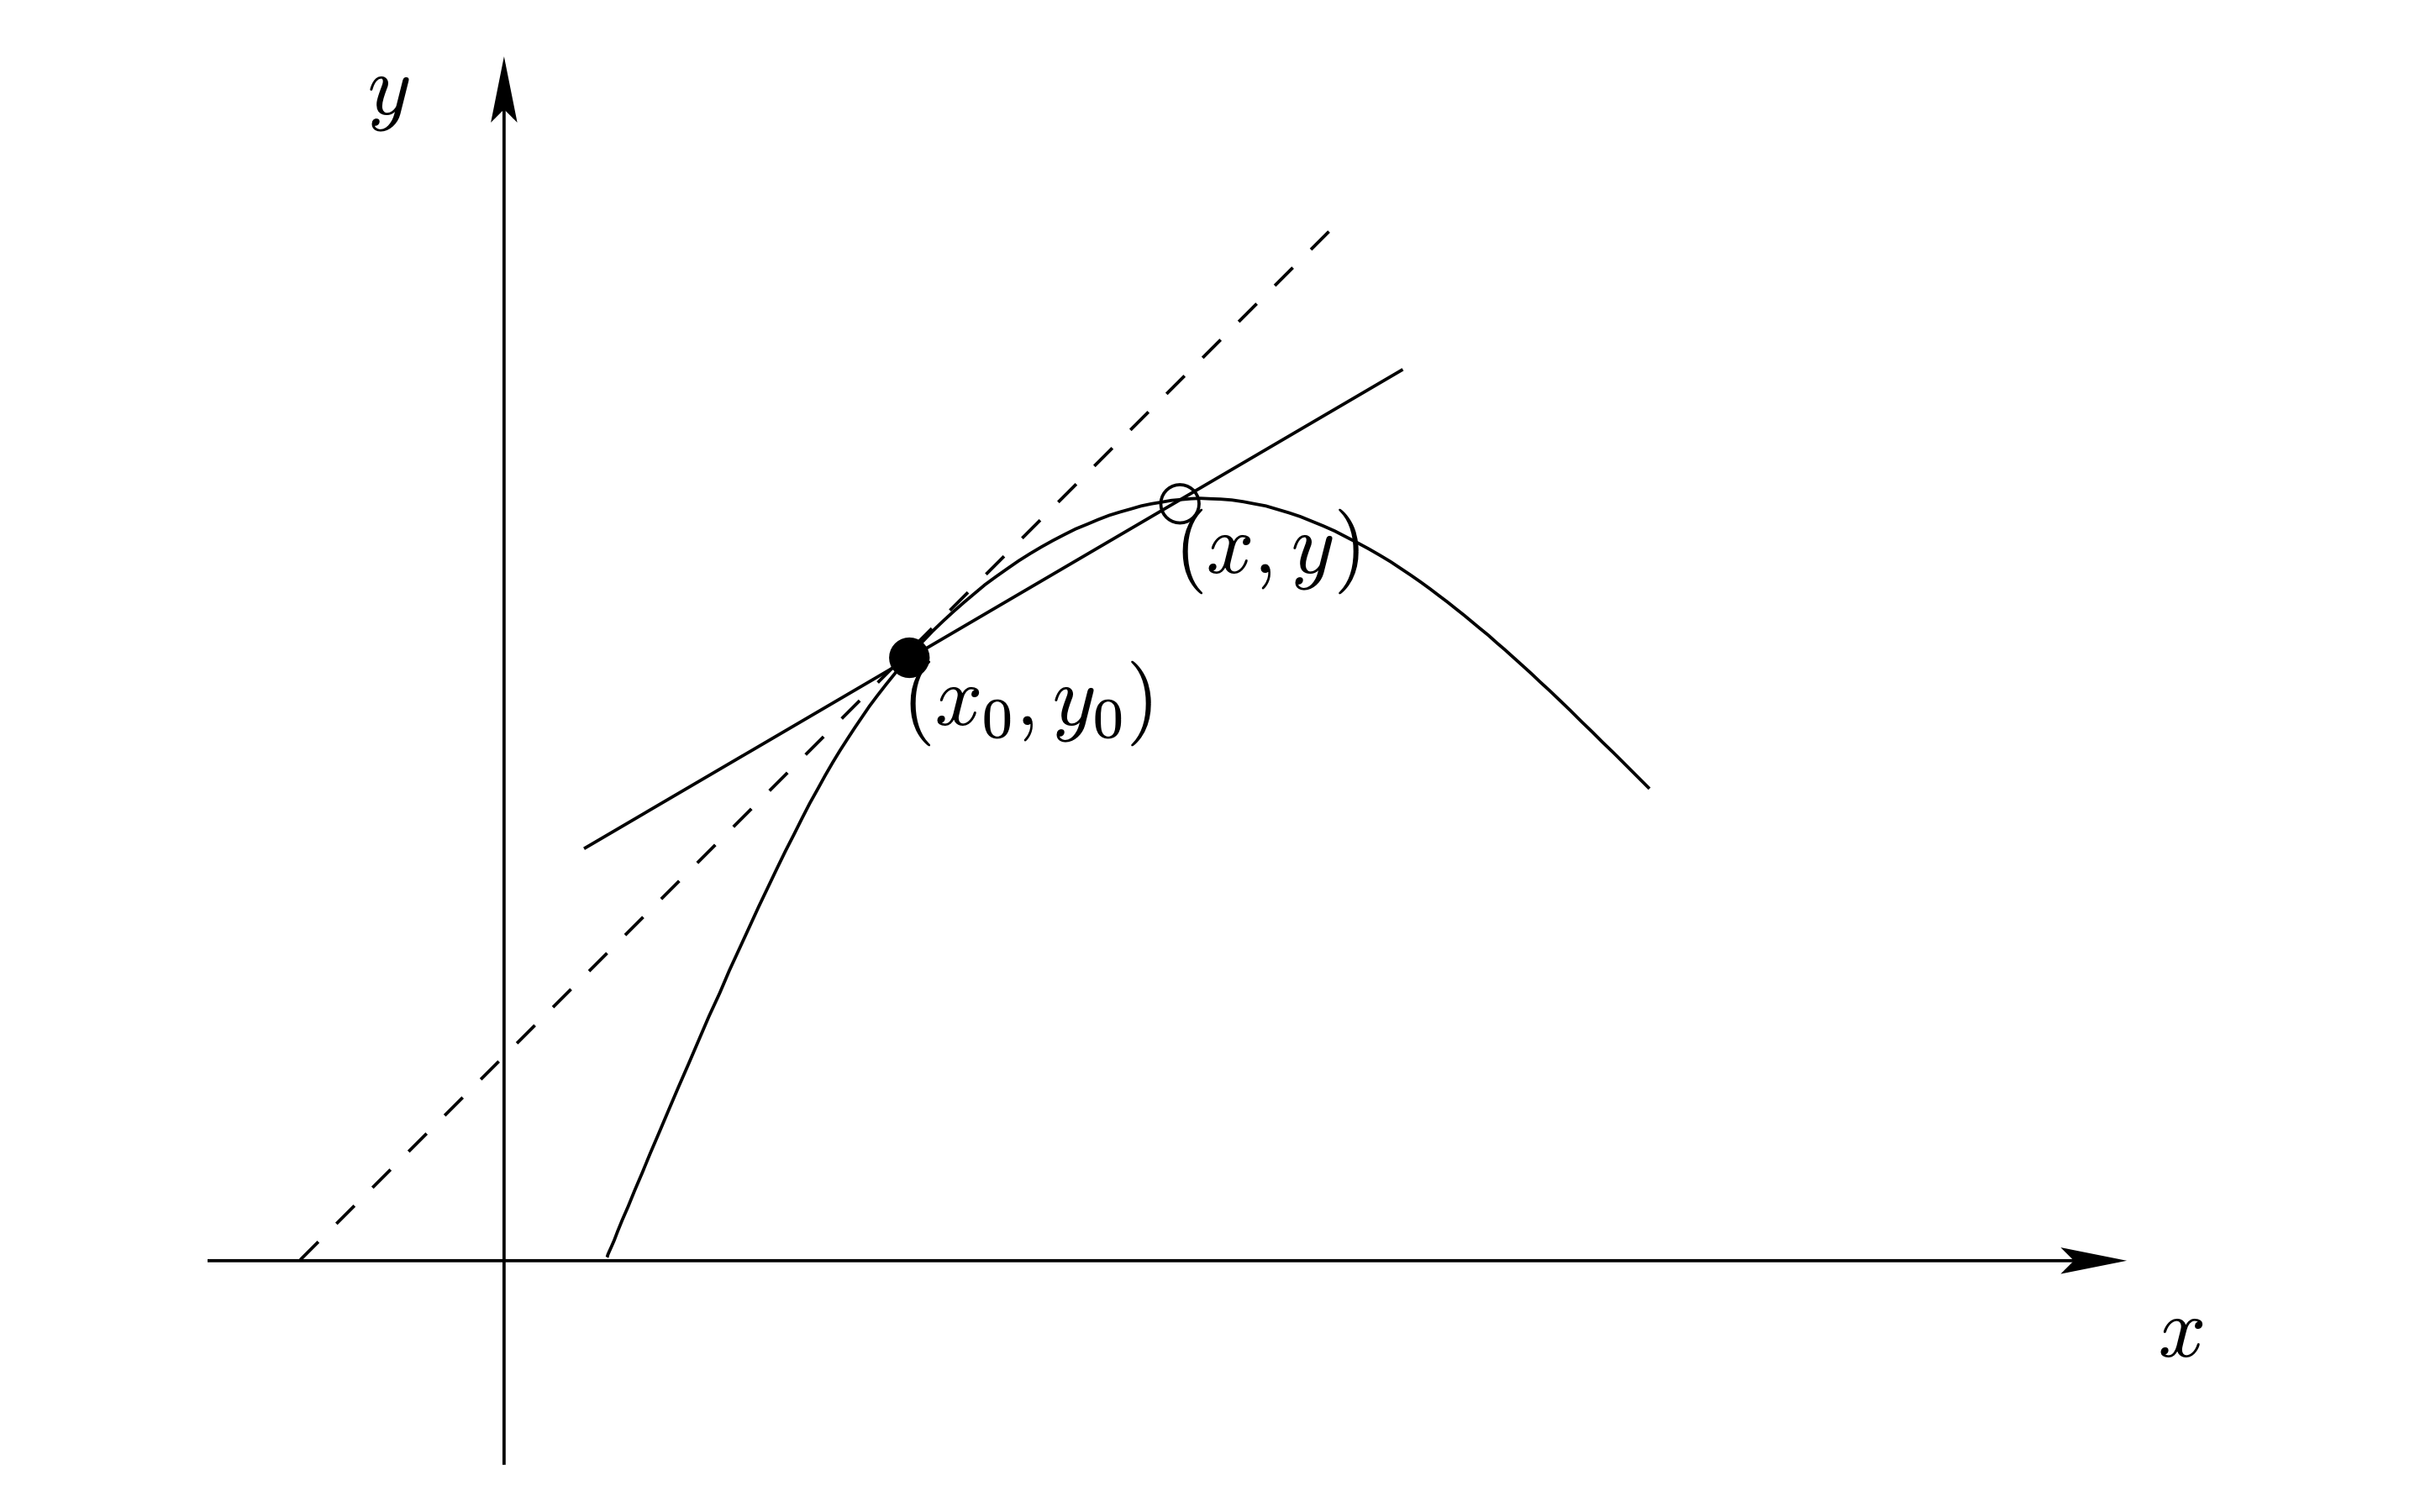
\includegraphics[width=0.5\linewidth]{images/fig-tangent-line} \caption{การหาเส้นตรงที่สัมผัสเส้นโค้ง}\label{fig:fig-tangent-line}
\end{figure}

ขั้นตอนสรุปการหาเส้นตรงที่สัมผัสเส้นโค้ง

\begin{enumerate}
\def\labelenumi{\arabic{enumi}.}
\item
  เลือกจุดอื่นบนกราฟ เรียกจุดนี้ว่า \(P(x,y)\)
\item
  ลากเส้นผ่าน \(PP_{0}\)
\item
  ทำซ้ำโดยเลือกจุด P ให้ใกล้ \(P_{0}\) มากขึ้น
\item
  เส้น \(PP_{0}\) ที่ได้จะ ``เข้าใกล้'' เส้นสัมผัสมากขึ้นทุกที
\end{enumerate}

\begin{itemize}
\tightlist
\item
  การหาพื้นที่ ``ใต้กราฟ'' ระหว่าง x = a กับ x = b
\end{itemize}

\begin{figure}
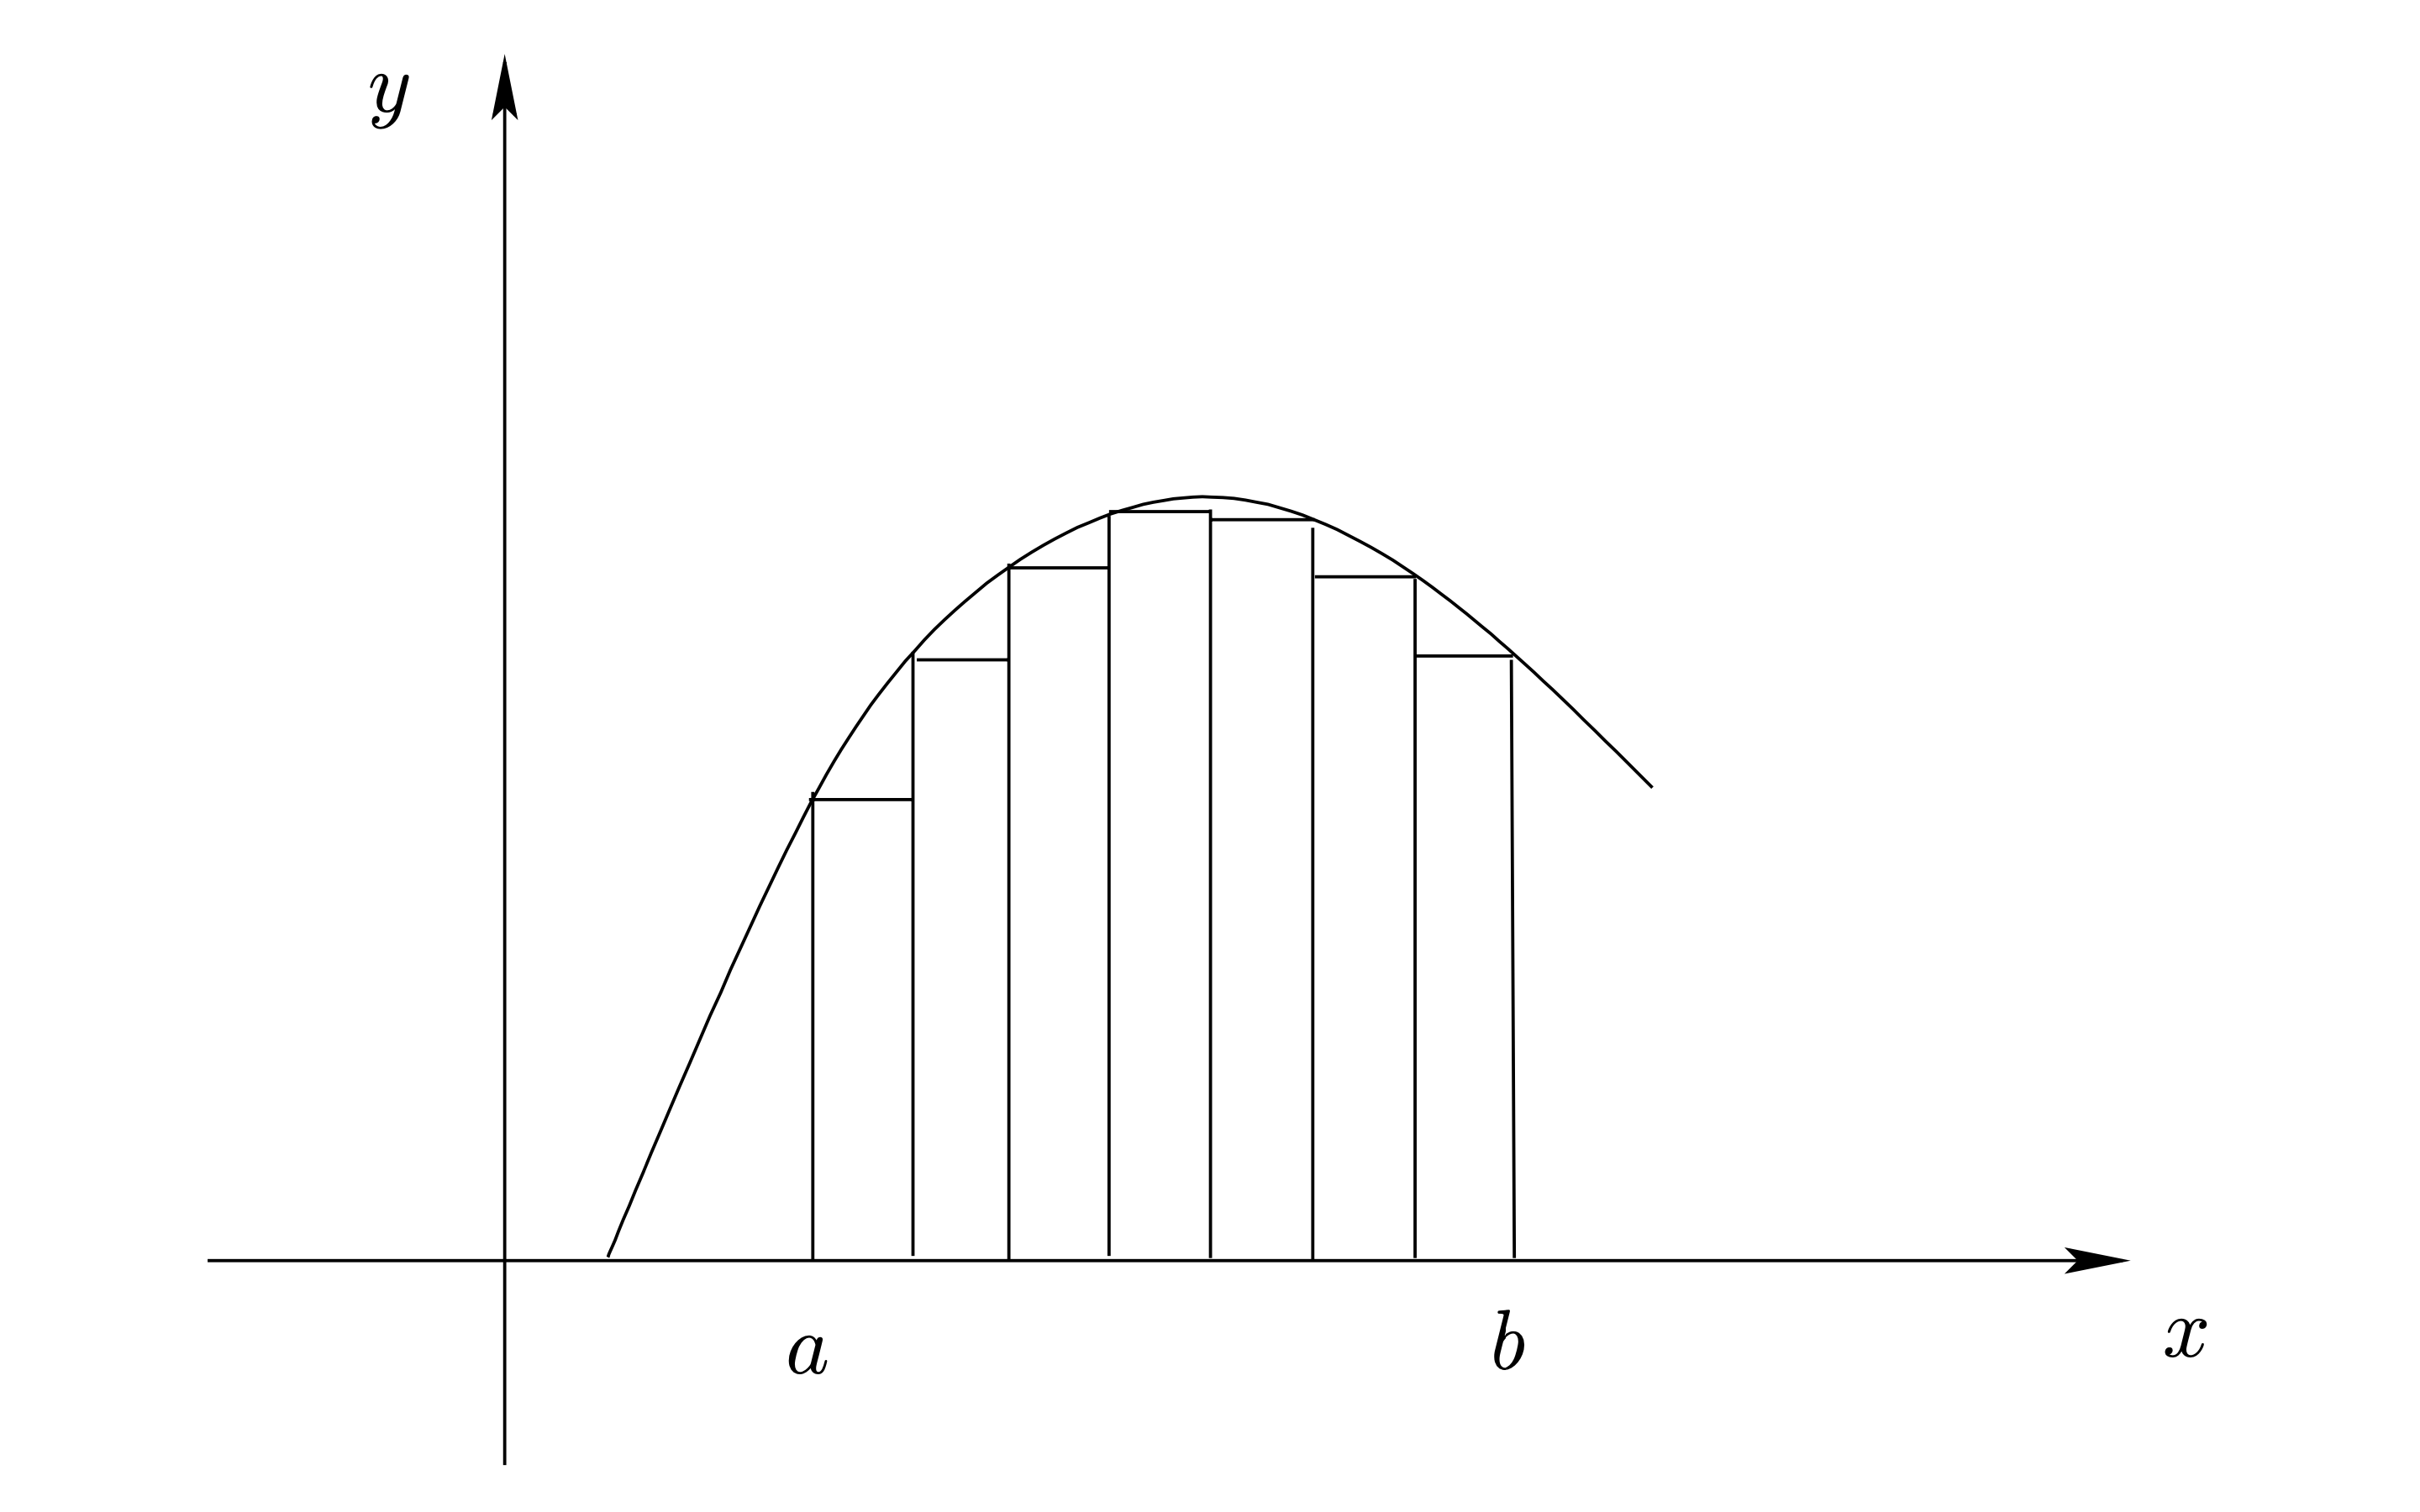
\includegraphics[width=0.5\linewidth]{images/fig-area-under-curve} \caption{การหาพื้นที่ใต้กราฟ}\label{fig:fig-area-under-curve}
\end{figure}

ขั้นตอนเบื้องต้นสำหรับการหาพื้นที่ใต้กราฟ

\begin{enumerate}
\def\labelenumi{\arabic{enumi}.}
\tightlist
\item
  แบ่ง \([a,b]\) เป็นช่วงเล็กๆ
\item
  หาพื้นที่รวมของสี่เหลี่ยมผืนผ้าทั้งหมด
\item
  ทำซ้ำๆ โดยแบ่งช่วงให้เล็กมากขึ้น
\item
  พื้นที่ที่ได้จะ ``เข้าใกล้'' พื้นที่ที่ต้องการมากขึ้นทุกที
\end{enumerate}

\phantomsection\label{ex-limit-1}
จงหาสมการของเส้นสัมผัสกราฟ \(y=-x^{2}+6x-2\) ณ จุด \(P_{0}(2,6)\)

\textbf{วิธีทำ} เลือกจุด \(P(x,y)\) โดยที่ \(x \neq 2\) และลากเส้น \(PP_{0}\)
จะได้ว่า ความชันของ \(PP_{0}\) เท่ากับ \[\begin{aligned}
    \frac{y-6}{x-2} &= \frac{-x^{2}+6x-8}{x-2} \\
                    &=-\frac{\left( x-2\right) \left( x-4\right) }{x-2} \\
                    &=4-x
\end{aligned}\] ถ้า \(P\) อยู่ใกล้ \(P_{0}\) มากขึ้น ค่า x ย่อมเกือบเป็น 2 ดังนั้น
ความชันของ \(PP_{0}\) จึงเข้าใกล้ 4-2 = 2 มากขึ้นเรื่อย ๆ เส้นสัมผัสจึงควรมีความชันเป็น
2 และสมการเส้นสัมผัส คือ \(y-6=2\left( x-2\right)\)

\begin{figure}
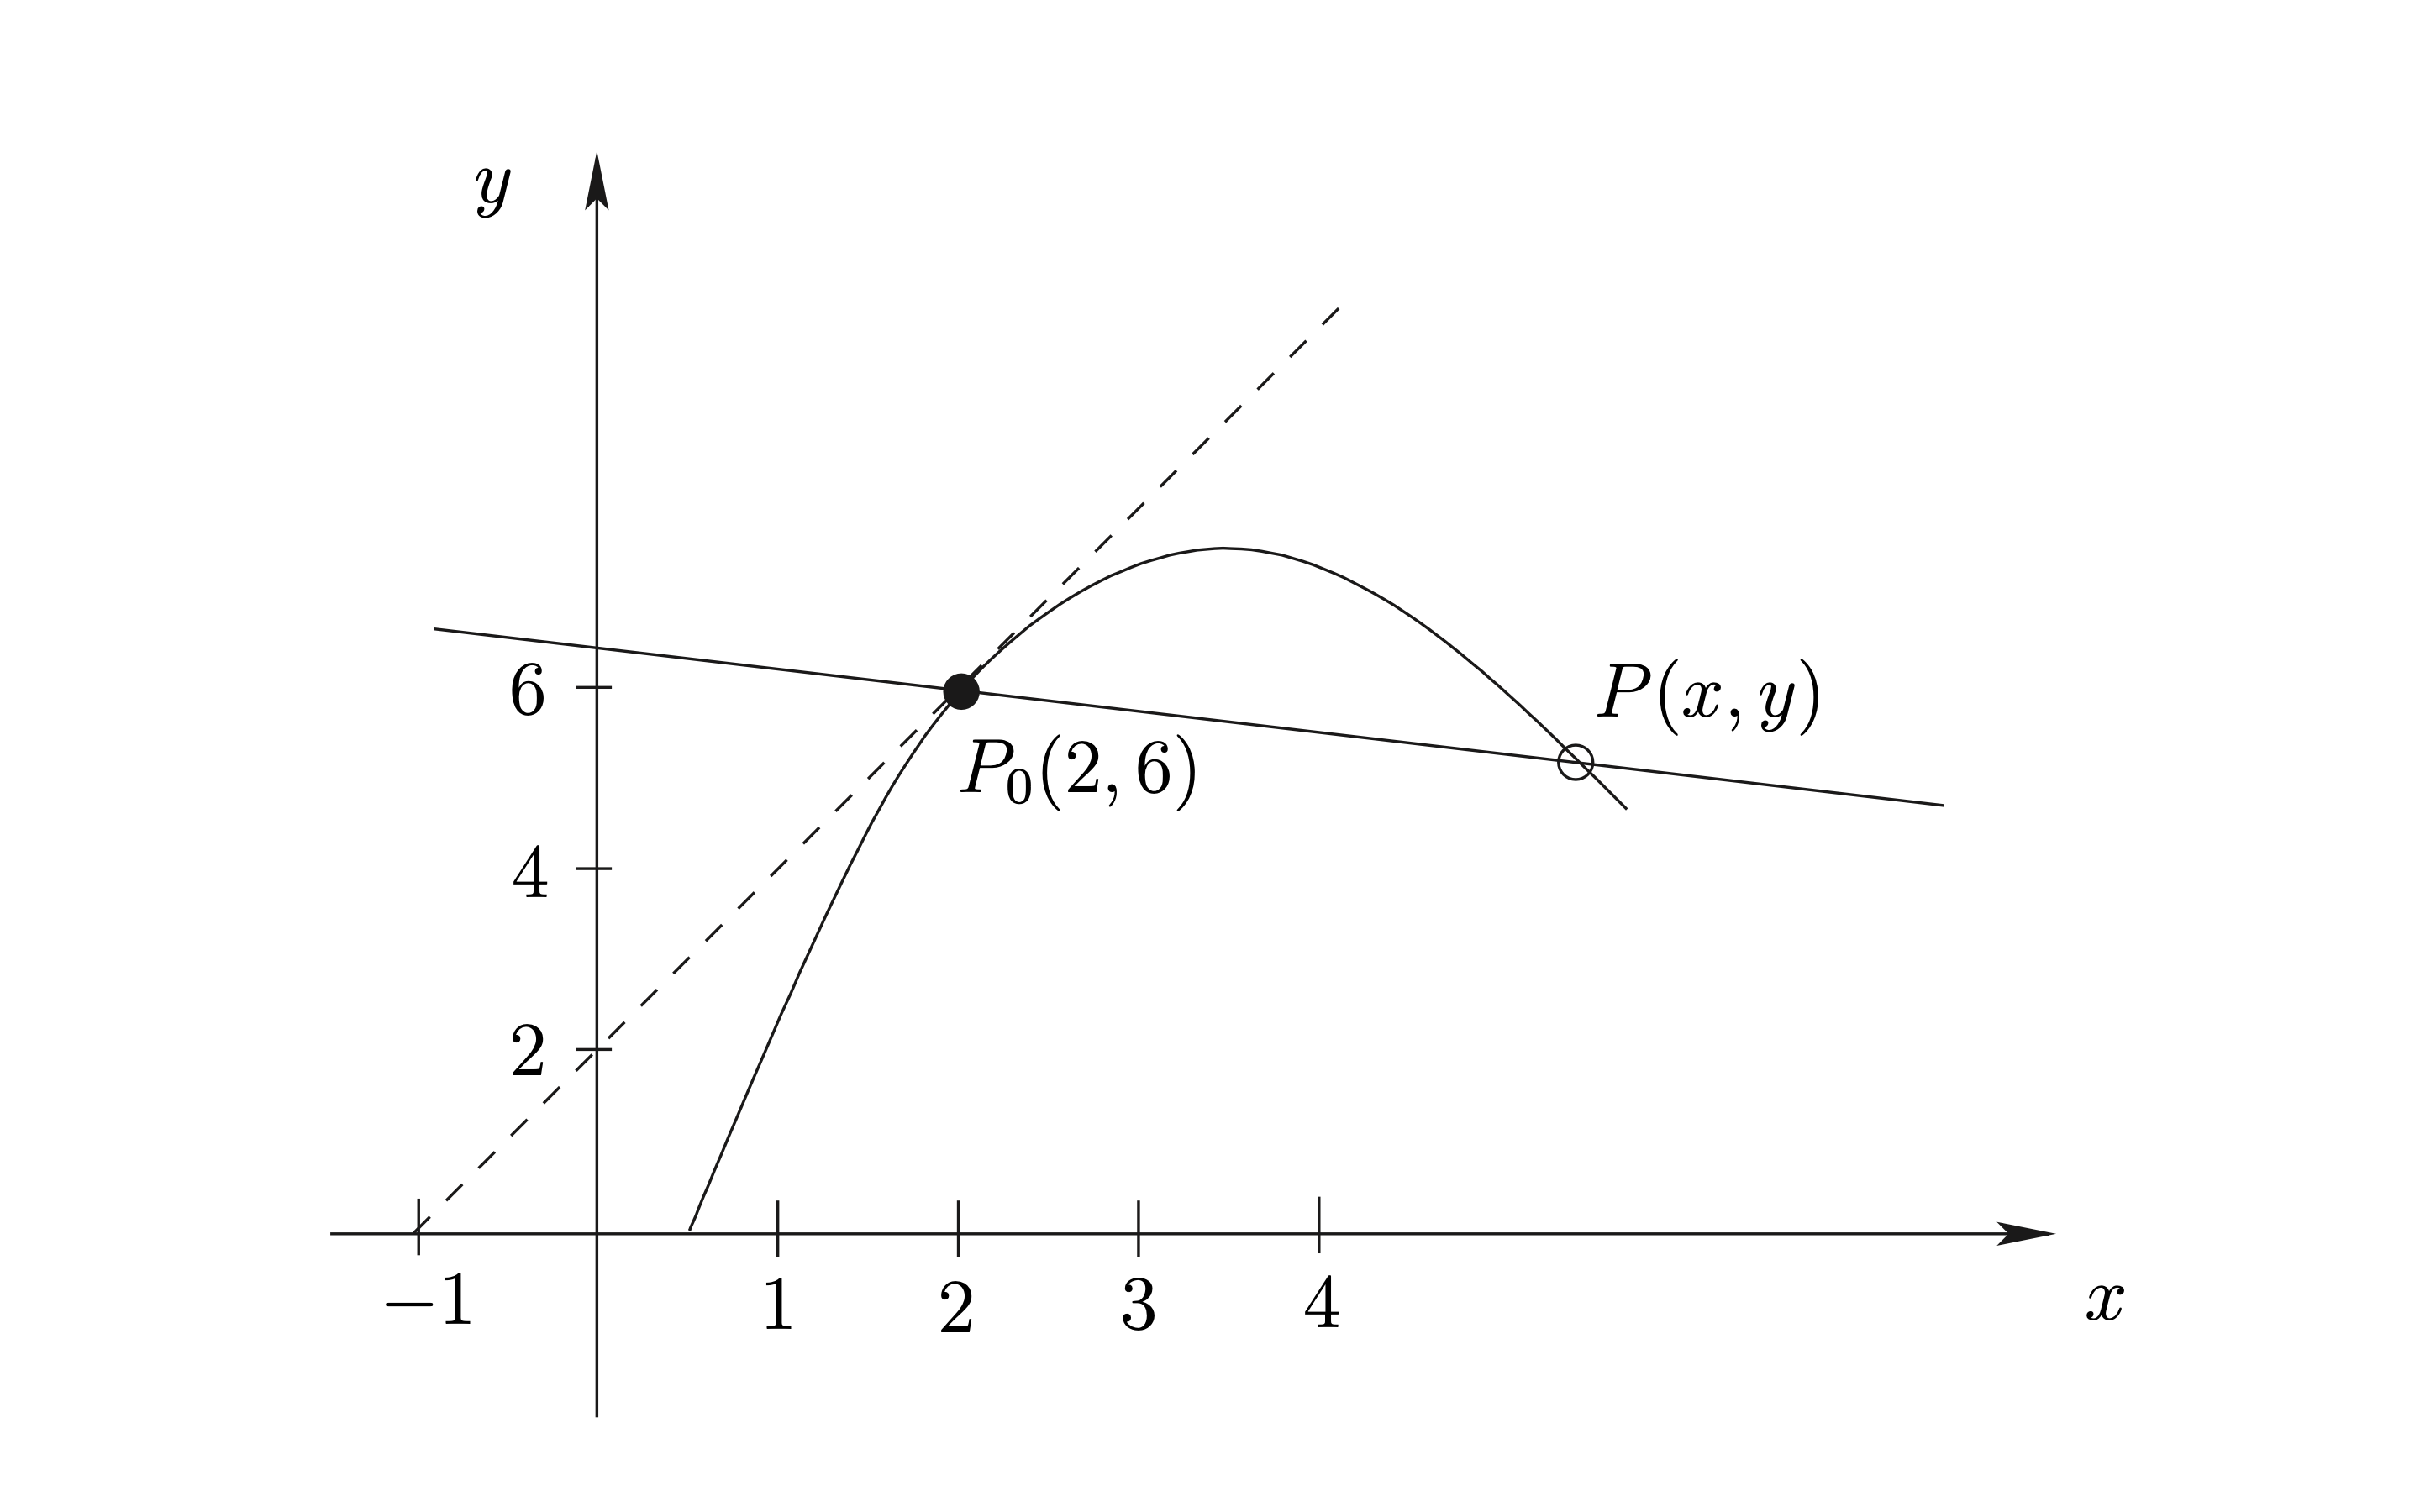
\includegraphics[width=0.5\linewidth]{images/fig-tangent-line-2} \caption{การหาเส้นตรงที่สัมผัสเส้นโค้ง \(y=-x^{2}+6x-2\)}\label{fig:fig-tangent-line-2}
\end{figure}

จะเห็นว่า ในตัวอย่าง @ref(exm:ex-limit-1) นี้ เราสนใจพฤติกรรมของ function

\(\frac{-x^{2}+6x-8}{x-2}\) เมื่อ \(x \neq 2\) แต่มีค่าใกล้ 2 มาก ๆ นี่คือ
ที่มาของเรื่อง

\phantomsection\label{def-limit}
ให้ \(f : D_{f}\rightarrow R\) โดยที่ \(D_{f}\subseteq R\) และให้
\(a \in R\) โดยที่มีช่วง \((a,b)\) บางช่วงที่
\(\left( a,b\right) \subseteq D_{f}\left( b>a\right)\)

เรากล่าวว่า "ลิมิต (limit) ของ \(f(x)\) เมื่อ x เข้าใกล้ a ทางขวา
หาค่าได้และมีค่าเท่ากับจำนวนจริง L" ถ้า "ไม่ว่าเราจะกำหนดบริเวณรอบ ๆ \(L\)
ไว้แคบเพียงใด เมื่อเราพิจารณาค่าของ \(f(x)\) สำหรับค่า \(x\) ที่มากกว่า a โดยที่ให้ค่า
ของ \(x\) ลดลงเรื่อย ๆ จนถีงจุดหนึ่ง ค่าของ \(f(x)\) จะอยู่ในบริเวณรอบ ๆ \(L\)
ที่เรากำหนดไว้นั้น และยังคงเป็นเช่นนี้สำหรับ \(x\) อื่น ๆ ที่น้อยกว่านั้น (แต่มากกว่า \(a\) )
ทั้งหมดด้วย"

ในทำนองเดียวกัน ถ้าเราพิจารณาพฤติกรรมของ function สำหรับ \(x\) ที่น้อยกว่า \(a\)
จะได้ limit ทางซ้าย ดังนี้ ให้ \(f : D_{f}\rightarrow R\) โดยที่
\(D_{f}\subseteq R\) และให้ \(a \in R\) โดยที่มีช่วง \((b,a)\) บางช่วงที่
\(\left( b,a\right) \subseteq D_{f}\left( b<a\right)\)

เรากล่าวว่า "limit ของ \(f(x)\) เมื่อ \(x\) เข้าใกล้ a ทางซ้าย หาค่าได้
และมีค่าเท่ากับจำนวนจริง \(L\)" ถ้า "ไม่ว่าเราจะกำหนดบริเวณรอบ ๆ \(L\)
ไว้แคบเพียงใด

เมื่อเราพิจารณาค่าของ \(f(x)\) สำหรับค่า \(x\) ที่น้อยกว่า \(a\) โดยที่ให้ค่า ของ
\(x\) เพิ่มขึ้นเรื่อย ๆ จนถีงจุดหนึ่ง ค่าของ \(f(x)\) จะอยู่ในบริเวณรอบ ๆ \(L\)
ที่เรากำหนดไว้นั้น และยังคงเป็นเช่นนี้สำหรับ \(x\) อื่น ๆ ที่มากกว่านั้น (แต่น้อยกว่า \(a\) )
ทั้งหมดด้วย"

เราใช้สัญลักษณ์ \(\underset{x\rightarrow a^{+}}{\lim}f(x)\) แทนข้อความ "limit
ของ \(f(x)\) เมื่อ \(x\) เข้าใกล้ a ทางขวา" และใช้สัญลักษณ์
\(\underset{x\rightarrow a^{-}}{\lim}f(x)\) แทนข้อความ "limit ของ
\(f(x)\) เมื่อ \(x\) เข้าใกล้ a ทางซ้าย

\phantomsection\label{def-limit-2}
ในกรณีที่ทั้ง \(\underset{x\rightarrow a^{+}}{\lim}f(x)\) และ
\(\underset{x\rightarrow a^{-}}{\lim}f(x)\) หาค่าได้ และมีค่าเท่ากัน

เรากล่าวว่า \(\underset{x\rightarrow a}{\lim}f(x)\) หาค่าได้ และมีค่าเท่ากับค่านั้น

\phantomsection\label{ex-limit-2}
function \(f\) ที่ \(\underset{x\rightarrow a^{+}}{\lim}f(x)\) หาค่าไม่ได้
ดังนั้น

\(\underset{x\rightarrow a}{\lim}f(x)\) จึงหาค่าไม่ได้ด้วย

\textbf{วิธีทำ} จากรูปต่อไปนี้

ในกรณีนี้ จะเห็นว่า ไม่ว่าจะเลือก \(L\) เป็นค่าใด ก็ไม่สามารถสรุปได้ว่า
\(\underset{x\rightarrow 0^{+}}{\lim}f(x)=L\)
เพราะไม่ใช่ทุกครั้งที่เรากำหนดบริเวณรอบ ๆ \(L\) แล้ว function
จะสอดคล้องตามนิยามเสมอไป จึงสรุปว่า \(\underset{x\rightarrow a}{\lim}f(x)=L\)
หาค่าไม่ได้ด้วย

\backmatter
\end{document}
